\subsection{Saddle Points}
\label{sec:sps}

Saddle points are stationary points, i.e. with zero gradient, on a multidimensional function, $f(\vR)$, that are neither maxima nor minima.

\begin{figure}[h]
  \begin{center}
    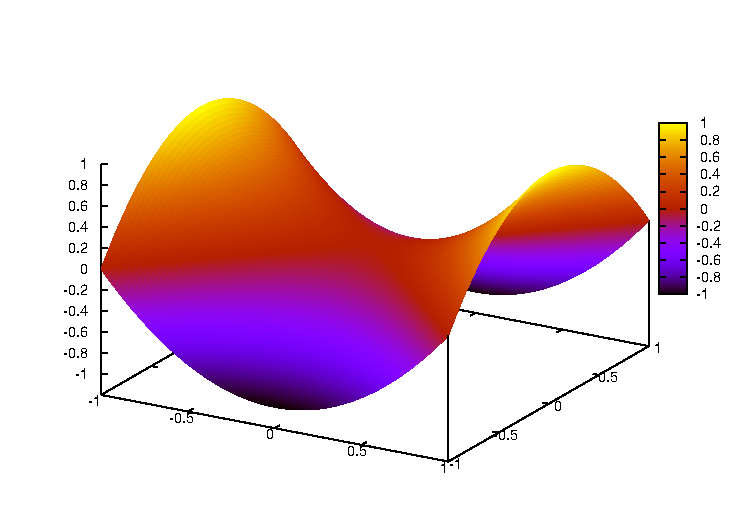
\includegraphics[width=0.6\linewidth]{saddle-point}
    \parbox{0.85\linewidth}{
      \caption{A first order saddle point.
      $f(x=0, y=0) = x^2 - y^2$. A minimum in the $x$ direction and a maximum in the $y$ direction.
      \figmiss{I'd like to have a saddle for horse riding as a comparison here.}
      \figmiss{1D: $f(x=0) = x^3$}
      }
      \label{fig:2d-saddle-point}
    }
  \end{center}
\end{figure}

A common view of a saddle (point) can be found in \fref{fig:2d-saddle-point} as the function $f(x, y) = x^2 - y^2$ which near $(x,y) = (0,0)$ resembles a saddle, used when riding horses, curving upwards in one direction and downwards in the other.
This image of a saddle point lacks a few elements to be to tell their whole story but acts as a good general case.
On functions of higher dimensionality than $2$, different orders of saddle points are possible.
The order of the saddle point is decided by the amount of directions that are not at a minimum, or the non-positive eigenvalues of the Hessian.
As such, \fref{fig:2d-saddle-point} shows a first order saddle point on a two dimensional function.
In this thesis, saddle points of order $N$ will be indicated by \sap{N} from here on.

The Hessian at the \sap{} displayed in \fref{fig:2d-saddle-point} has one negative eigenvalue, however, a saddle point with one or more vanishing eigenvalues is also possible, such as the 1D example $f(x = 0) = x^3$, as seen in \fref{fig:1d-saddle-point}.

Locating \sap{}s in multiple dimensions is a non-trivial task as only a limited number of steepest decent paths lead to each one while the majority lead to minima.
A number of schemes have been suggested~\citemiss, two popular ones are discussed below, in \fref{sec:saddle-point-methods}: The Dimer method and the Nudged Elastic Band method.

